Os trabalhos que propõem soluções para o descarregamento de tarefas em redes veiculares frequentemente adotam uma premissa simplificadora na modelagem do sistema computacional: a construção do ambiente de simulação baseada em modelos analíticos determinísticos. Um exemplo típico é o cálculo do tempo de processamento definido como a razão entre os ciclos computacionais requeridos e a frequência de \gls{CPU} disponível, somado ao emprego de modelos de consumo energético fundamentados na potência dinâmica e em aproximações derivadas \cite{rabaey2003digital,mao2016dynamic}.

Embora essas escolhas tornem o problema tratável e facilitem a comparação de algoritmos em condições controladas, elas tendem a limitar a fidelidade ao representar o ambiente dinâmico das redes veiculares. Adicionalmente, a derivação direta de uma grandeza a partir de outra cria uma forte correlação entre o tempo de processamento e o consumo energético. Tal situação mostra-se problemática na prática, uma vez que análises estatísticas como regressão linear, \gls{PCA} e certos algoritmos de aprendizado requerem matrizes de covariância bem condicionadas, requisito não satisfeito quando há alta colinearidade entre as variáveis preditoras \cite{montgomery2021introduction}. Se a energia consumida for estritamente proporcional ao tempo de processamento, torna-se inviável distinguir o impacto individual de cada variável no desempenho do sistema.

Para ilustrar essa questão, considere o modelo usual para calcular o tempo de processamento (Equação \ref{fm:tempo-processamento}) e o consumo energético (Equação \ref{fm:consumo-energetico}) de uma tarefa $i$ em um nó $j$:
\begin{equation}
T_{i,j}^{\text{proc}} = \frac{C_i}{f_j}
\label{fm:tempo-processamento}
\end{equation}
\begin{equation}
E_{i,j}^{\text{proc}} = \kappa_j f_j^2 C_i
\label{fm:consumo-energetico}
\end{equation}
\noindent onde $C_i$ representa o número de ciclos computacionais necessários para processar a tarefa $i$, $f_j$ é a frequência do processador do nó $j$, e $\kappa_j$ é uma constante de consumo energético dependente da capacitância efetiva da arquitetura do nó $j$. Observe que, a partir da Equação \ref{fm:tempo-processamento}, obtém-se:
\begin{equation}
C_i = T_{i,j}^{\text{proc}} f_j
\label{fm:c-em-funcao-de-t-proc}
\end{equation}
\noindent e, ao substituirmos em (\ref{fm:consumo-energetico}), tem-se:
\begin{equation}
E_{i,j}^{\text{proc}} = \kappa_j f_j^2 (T_{i,j}^{\text{proc}} f_j) = \kappa_j f_j^3 T_{i,j}^{\text{proc}}
\label{fm:consumo-energetico-em-funcao-de-c}
\end{equation}
Dessa forma, $E_{i,j}^{\text{proc}}$ torna-se uma função linear de $T_{i,j}^{\text{proc}}$ ao se fixarem os valores de $\kappa_j$ e $f_j$, estabelecendo uma correlação perfeita entre as grandezas. A Tabela \ref{tab:correlacao-energia-tempo} exemplifica esse comportamento assumindo $\kappa_j = 10^{-27}$ e $f_j=2$ GHz; a Figura \ref{fig:perfect_collinearity} ilustra graficamente esta relação.
\begin{table}[ht!]	
    \centering
    \Caption{\label{tab:correlacao-energia-tempo} Correlação entre tempo de processamento e consumo energético em um cenário típico de simulação}
    \UECEtab{}{
        \begin{tabular}{clll}
            \toprule
            Tarefa & $C$ (ciclos) & $T^{\text{proc}}$ (ms) & $E^{\text{proc}}$ (mJ) \\
            \midrule \midrule
            1 & $2 \times 10^6$ & 1.0 & 8.0 \\
            2 & $5 \times 10^6$ & 2.5 & 20.0 \\
            3 & $1 \times 10^6$ & 0.5 & 4.0 \\
            4 & $8 \times 10^6$ & 4.0 & 32.0 \\
            5 & $3 \times 10^6$ & 1.5 & 12.0 \\
            \bottomrule
        \end{tabular}
    }{
    \Fonte{Elaborado pelo autor}
}
\end{table}

\begin{figure}[ht!]
    \centering
    \Caption{\label{fig:perfect_collinearity} O gráfico ilustra a colinearidade perfeita: todos os pontos alinham-se em uma reta, indicando que uma variável é redundante em relação à outra.}
    \UECEfig{}{
        \begin{tikzpicture}
            \draw[->] (0,0) -- (5,0) node[right] {$T^{\text{proc}}$ (ms)};
            \draw[->] (0,0) -- (0,5) node[above] {$E^{\text{proc}}$ (mJ)};
            
            % Perfect line
            \draw[blue, thick] (0,0) -- (4.5, 4.5);
            
            % Points exactly on the line
            \fill[red] (0.5, 0.5) circle (2pt) node[above right, font=\tiny] {Tarefa 1};
            \fill[red] (1.0, 1.0) circle (2pt) node[above right, font=\tiny] {Tarefa 3};
            \fill[red] (1.5, 1.5) circle (2pt) node[above right, font=\tiny] {Tarefa 5};
            \fill[red] (2.5, 2.5) circle (2pt) node[above right, font=\tiny] {Tarefa 2};
            \fill[red] (4.0, 4.0) circle (2pt) node[above right, font=\tiny] {Tarefa 4};
            
            \node[blue, rotate=45] at (2.5, 3.2) {$E = 8 \cdot T^{\text{proc}}$};
        \end{tikzpicture}
    }{
        \Fonte{Elaborado pelo autor}
    }
\end{figure}

A partir dos resultados, infere-se que $E_{i,j}^{\text{proc}} = 8 \times T_{i,j}^{\text{proc}}$. O cálculo da correlação de Pearson entre as duas séries da Tabela \ref{tab:correlacao-energia-tempo} resulta em $\widehat{\mathrm{Corr}}(T_{\text{proc}}, E_{\text{proc}})=1$, confirmando a colinearidade perfeita. Isso implica que as variáveis carecem de independência estatística, ou seja, apresentam redundância informacional completa. Consequentemente, o uso de modelos de sistema excessivamente simplificados (por exemplo, assumindo $\kappa_j$ e $f_j$ constantes no tempo) deve ser realizado com cautela, pois pode mascarar \textit{trade-offs} relevantes entre atraso e energia, levando a conclusões imprecisas sobre o desempenho das soluções de decisão de descarregamento de tarefas.

Outra simplificação frequente reside na geração da carga de trabalho. Em muitos ambientes simulados, a chegada de tarefas segue processos de \textit{Poisson}, enquanto atributos como tamanho, densidade computacional e prazos (\textit{deadlines}) são definidos a partir de distribuições uniformes ou normais. Embora útil para testes iniciais, essa prática não descreve adequadamente a variabilidade dos cenários reais, onde a demanda flutua conforme o contexto. Empiricamente, a validade da hipótese de chegadas puramente \textit{Poisson} é contestada em redes de dados reais, falhando em capturar a variabilidade do tráfego em grandes escalas \cite{paxson1995wide}. 

% Tais ambientes são caracterizados pela presença de tráfego bem comportado e autossimilaridade, exibindo dependência temporal de longa duração que modelos sem memória não conseguem reproduzir \cite{leland1994self}, o que motiva a adoção de modelos de tráfego mais sofisticados \cite{li2019compound}.

Formalmente, a execução de uma simulação gera séries temporais que descrevem a evolução das variáveis do sistema (e.g., taxa de chegada, carga do processador). Nesse contexto, uma série é dita \textbf{estacionária} quando suas propriedades estatísticas fundamentais, como média e variância, permanecem constantes ao longo do tempo \cite{hyndman2021fpp3}. Por outro lado, traços \textbf{não estacionários} exibem alterações nessas propriedades, manifestando-se como tendências, mudanças de variância ou alternância entre regimes distintos.

Como resultado, cenários construídos exclusivamente sobre médias e desvios-padrão fixos (ou amostragens i.i.d.\ sem memória) falham em refletir a complexidade do mundo real. Contudo, em cenários não estacionários, é possível representar fenômenos comuns, como: picos e vales de demanda; degradação variável do canal devido à mobilidade; e flutuações no tempo de processamento causadas por contenção de recursos. Em síntese, a não estacionariedade é um fator que altera fundamentalmente a complexidade do problema, devendo ser um requisito central em avaliações realistas \cite{ahmed2022survey,3gpp38901}.

Diante disso, soluções para descarregamento de tarefas deveriam ser avaliadas preferencialmente em ambientes não estacionários, onde as condições variam ao longo do tempo em fases de comportamento persistentes. Uma abordagem controlável para introduzir esse comportamento é empregar modelos com mudança de regime, nos quais um processo de estados discretos governa, por intervalos de tempo, diferentes níveis de carga e condições operacionais \cite{hamilton1989,fischer1993mmpp,heffes1986mmpp}. 

Em redes, essa técnica é amplamente utilizada para capturar rajadas (\textit{burstiness}) e correlações temporais em tráfego e qualidade de enlace, por meio de modelos Markov-modulados (p.ex., MMPP e variações do modelo de Gilbert--Elliott) \cite{heffes1986mmpp,fischer1993mmpp,elliott1963}. No contexto de computação de borda, os regimes podem representar, de forma unificada, faixas para parâmetros de tarefa e condições de recursos computacionais e energéticos, evitando que o cenário se reduza a amostragens independentes. A Figura \ref{fig:regime_step_sem_inercia} exemplifica uma trajetória de regimes típica.

\begin{figure}[ht!]
    \centering
    \Caption{\label{fig:regime_step_sem_inercia} Exemplo de trajetória de regimes $Z(t)$ ao longo do tempo (sinal em degraus). Cada patamar representa um tempo de permanência no regime; as transições representam mudanças de fase (Markov-modulado).}
    \UECEfig{}{
        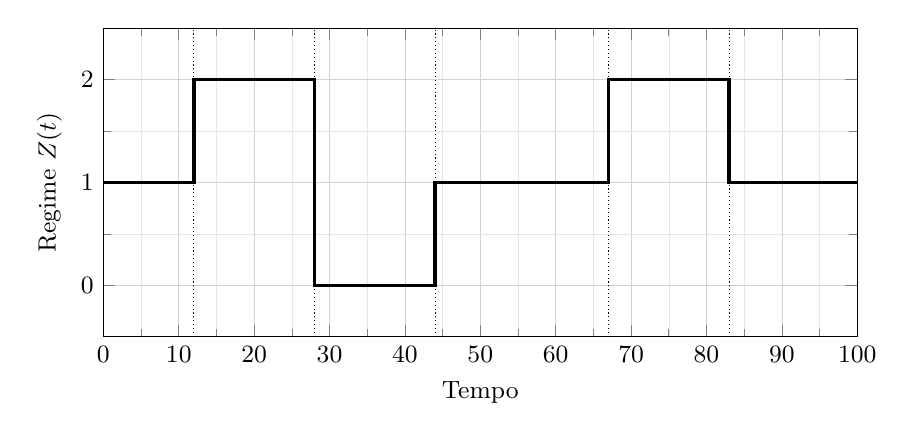
\begin{tikzpicture}
            \begin{axis}[
              width=0.92\linewidth,
              height=5.5cm,
              xmin=0, xmax=100,
              ymin=-0.5, ymax=2.5,
              xlabel={Tempo},
              ylabel={Regime $Z(t)$},
              ytick={0,1,2},
              yticklabels={0,1,2},
              grid=both,
              major grid style={line width=.2pt, draw=gray!35},
              minor grid style={line width=.1pt, draw=gray!20},
              minor tick num=1,
              ticklabel style={font=\small},
              label style={font=\small},
            ]
            % Regime in steps (example path)
            \addplot[
              const plot,
              line width=1.2pt
            ] coordinates {
              (0,1)   (12,1)
              (12,2)  (28,2)
              (28,0)  (44,0)
              (44,1)  (67,1)
              (67,2)  (83,2)
              (83,1)  (100,1)
            };
            % Optional vertical markers at switches (makes "dwell times" explicit)
            \addplot[densely dotted] coordinates {(12,-0.5) (12,2.5)};
            \addplot[densely dotted] coordinates {(28,-0.5) (28,2.5)};
            \addplot[densely dotted] coordinates {(44,-0.5) (44,2.5)};
            \addplot[densely dotted] coordinates {(67,-0.5) (67,2.5)};
            \addplot[densely dotted] coordinates {(83,-0.5) (83,2.5)};
            \end{axis}
        \end{tikzpicture}
    }{
        \Fonte{Elaborado pelo autor}
    }
\end{figure}

Esse procedimento também mitiga o problema de colinearidade discutido anteriormente. Ao permitir que $\kappa(t)$ e $f(t)$ evoluam como processos com regimes próprios e escalas de tempo distintas, o consumo energético deixa de ser um simples reescalonamento do tempo de processamento. O simulador passa a produzir um cenário onde tempo e energia são correlacionados mas não redundantes, aproximando-se de situações reais onde o escalonamento do sistema operacional e a heterogeneidade do hardware introduzem variabilidade independente.

Além disso, para evitar mudanças instantâneas irreais nas variáveis físicas, é desejável impor inércia ao sistema por meio de uma dinâmica de primeira ordem. Formalmente, define-se $u(t)$ como o valor alvo imposto pelo regime (sinal em degraus) e $y(t)$ como a resposta observável do sistema. A evolução temporal de $y(t)$ pode ser descrita pela equação de recorrência $y_{k+1} = \alpha y_k + (1-\alpha)u_k$, onde $\alpha \in [0,1)$ é o fator de inércia que controla a suavidade da transição, conforme ilustrado na Figura \ref{fig:regime_com_inercia}. Essa escolha é consistente com a prática de modelagem em arquitetura de computadores, onde a evolução de grandezas agregadas (como a temperatura) é representada por redes equivalentes de resistências e capacitâncias (modelos RC), que induzem uma resposta suavizada no tempo \cite{skadron2003hotspot}.

\begin{figure}[ht!]
    \centering
    \Caption{\label{fig:regime_com_inercia} Mesmo regime da Figura \ref{fig:regime_step_sem_inercia}, agora mapeado para um alvo $u(t)$ (degraus) e para uma variável observável $y(t)$ que responde com inércia de primeira ordem (rampas suaves).}
    \UECEfig{}{
        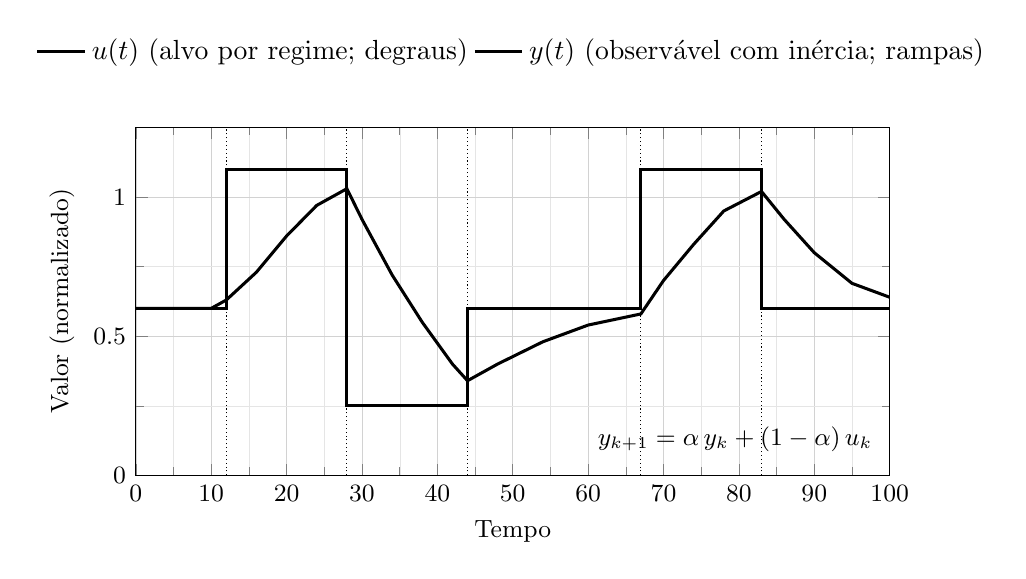
\begin{tikzpicture}
            \begin{axis}[
              width=0.92\linewidth,
              height=6.0cm,
              xmin=0, xmax=100,
              ymin=0, ymax=1.25,
              xlabel={Tempo},
              ylabel={Valor (normalizado)},
              grid=both,
              major grid style={line width=.2pt, draw=gray!35},
              minor grid style={line width=.1pt, draw=gray!20},
              minor tick num=1,
              legend style={at={(0.5,1.15)}, anchor=south, legend columns=2, draw=none, fill=none},
              ticklabel style={font=\small},
              label style={font=\small},
            ]
            % u(t): regime targets in steps (aligned with Fig 1 switch times)
            \addplot[
              const plot,
              line width=1.1pt
            ] coordinates {
              (0,0.60)  (12,0.60)
              (12,1.10) (28,1.10)
              (28,0.25) (44,0.25)
              (44,0.60) (67,0.60)
              (67,1.10) (83,1.10)
              (83,0.60) (100,0.60)
            };
            \addlegendentry{$u(t)$ (alvo por regime; degraus)}
            % y(t): inertial response (hand-crafted illustrative points)
            \addplot[
              line width=1.1pt
            ] coordinates {
              (0,0.60) (6,0.60) (10,0.60)
              (12,0.63) (16,0.73) (20,0.86) (24,0.97) (28,1.03)
              (30,0.92) (34,0.72) (38,0.55) (42,0.40) (44,0.34)
              (48,0.40) (54,0.48) (60,0.54) (67,0.58)
              (70,0.70) (74,0.83) (78,0.95) (83,1.02)
              (86,0.92) (90,0.80) (95,0.69) (100,0.64)
            };
            \addlegendentry{$y(t)$ (observável com inércia; rampas)}
            % switch markers (same as Fig 1)
            \addplot[densely dotted] coordinates {(12,0) (12,1.25)};
            \addplot[densely dotted] coordinates {(28,0) (28,1.25)};
            \addplot[densely dotted] coordinates {(44,0) (44,1.25)};
            \addplot[densely dotted] coordinates {(67,0) (67,1.25)};
            \addplot[densely dotted] coordinates {(83,0) (83,1.25)};
            \node[anchor=south east, font=\small] at (axis cs:99,0.05)
            {$y_{k+1}=\alpha\,y_k+(1-\alpha)\,u_k$};
            \end{axis}
        \end{tikzpicture}
    }{
        \Fonte{Elaborado pelo autor}
    }
\end{figure}

Por fim, do ponto de vista experimental, essa construção mantém a controlabilidade do cenário — via matrizes de transição e tempos de permanência — ao mesmo tempo que evita a validação em um ambiente estático. Torna-se possível, assim, avaliar políticas de \textit{task offloading} sob mudanças de fase coerentes, alinhando a simulação à dinâmica das redes veiculares.